\documentclass[a4paper]{article}
\usepackage[dutch]{babel}
\usepackage{eurosym}
\usepackage{hyperref}
\usepackage{graphicx}
\usepackage{amsmath}

\begin{document}

\section{Analyse oude syteem}
In dit hoofdstuk worden de mechanische aspecten en responsie van het oude mechanisme afgeleid en behandeld. Aan het einde van dit hoofdstuk worden conclusies getrokken over de sterke en zwakke punten van het huidige systeem.

\subsection{Algemene informatie}
(plaatje van opstelling met maten(SW)) \\
Zoals hierboven te zien is, bestaat de huidige rechtgeleiding uit twee verschillende bladveren met maten respectievelijk (lxbxh) ,van \textbf{()} die samen ervoor zorgen dat de rechtgeleiding met een bepaalde slag kan bewegen. Verder valt gelijk op te merken dat door het gebruik van twee bladveren het systeem overbepaald is.

\subsection{Systeemresponsie}
Met behulp van een van de beschikbaar gestelde opstellingen (opstelling 12) is de stapresponsie \textbf{(afbeelding)} bepaald met behulp van een blokvormig signaal
%\begin{figure}[h]
%\caption{Het gebruikte blokvormig signaal}
%  \centering
 %   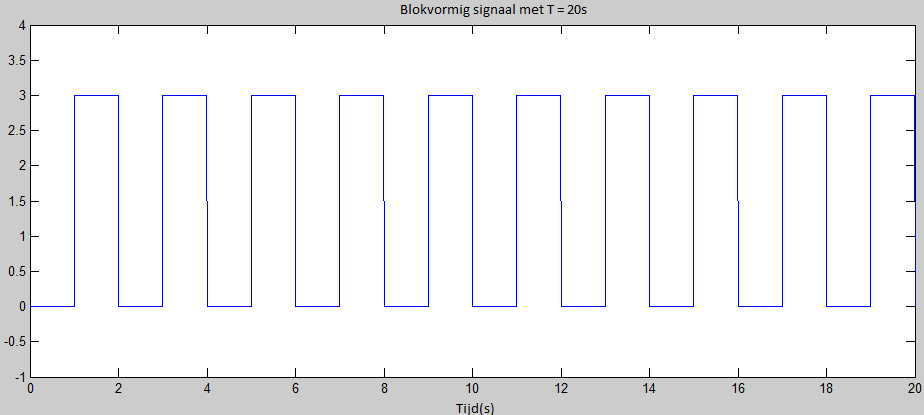
\includegraphics[width=0.5\textwidth]{Inputsignaal.png}
%\end{figure}

%\begin{figure}[h]
%\caption{Representatieve stapresponsie met data-markers}
%  \centering
 %   \includegraphics[width=0.5\textwidth]{Stapresponsie.png}
%\end{figure}

Het bestaande systeem kan benaderd worden met een gedempt massa-veersysteem, De responsie van dit systeem kan vervolgens gemodeleerd worden met een tweede orde overdrachtsfunctie. 
\begin{equation}
G(s) = K * \frac{\omega_n^2}{s^2 + 2 \zeta \omega_n s + \omega_n^2}
\end{equation}
Met behulp van de overshoot en de peak-time die te bepalen zijn uit afbeelding \textbf{(Stapresponsie)} kunnen $\zeta$, $\omega_n$ en de versterking $K$ bepaalt worden.
\begin{equation}
\zeta = \frac{1}{\sqrt{1 + (\frac{\pi}{\ln(OS})^2}} \ \ \ with \ \ OS = \frac{x(t_p)}{x(\infty)} -1
\end{equation}
\begin{equation}
\omega_n = \frac{\pi}{t_p \sqrt{1 - \zeta^2}} \ \ derived \ from \ \ \omega_d = \frac{\pi}{t_p} \ \ and \ \ \omega_d = \omega_n \sqrt{1-\zeta^2}
\end{equation}
\begin{equation}
K = \frac{x_{response}(\infty)}{x_{signal}(\infty)}
\end{equation}
De waarden voor $K$, $\zeta$ en $\omega_n$ zijn dus gelijk aan: $ K = 622$, 
$\zeta = 0.223$ en $\omega_n = 89.5 \frac{rad}{s} = 14.2 \ Hz$.\\
De overdrachtsfunctie van dit systeem wordt dus gelijk aan:
\begin{equation}
G(s) = 622 * \frac{8013}{s^2 + 39.86 s + 8013}
\end{equation}
(plaatje) \\
Als afbeeldingen (stapresponsie en overdrachtres) met elkaar vergeleken worden word bevestigd dat de berekende overdrachtsfunctie een goede benadering is van dit systeem. 

\subsection{Mechanische constanten}

\subsection{Eigenfrequenties}

\subsection{Conclusies en aanbevelingen}

\end{document}
